Poniższe obrazy uzyskano dla wartości współczynnika skupienia $e=128$ dla modelu Blinna-Phonga oraz $e=1024$ w przypadku modelu Torrance'a-Sparrowa - różnica ta opiera się na obserwacji, że model Torrance'a-Sparrowa generuje znacznie słabsze rozbłyski, dla takich samych wartości $e$.

\begin{figure}[H]
\centering
\subfigure{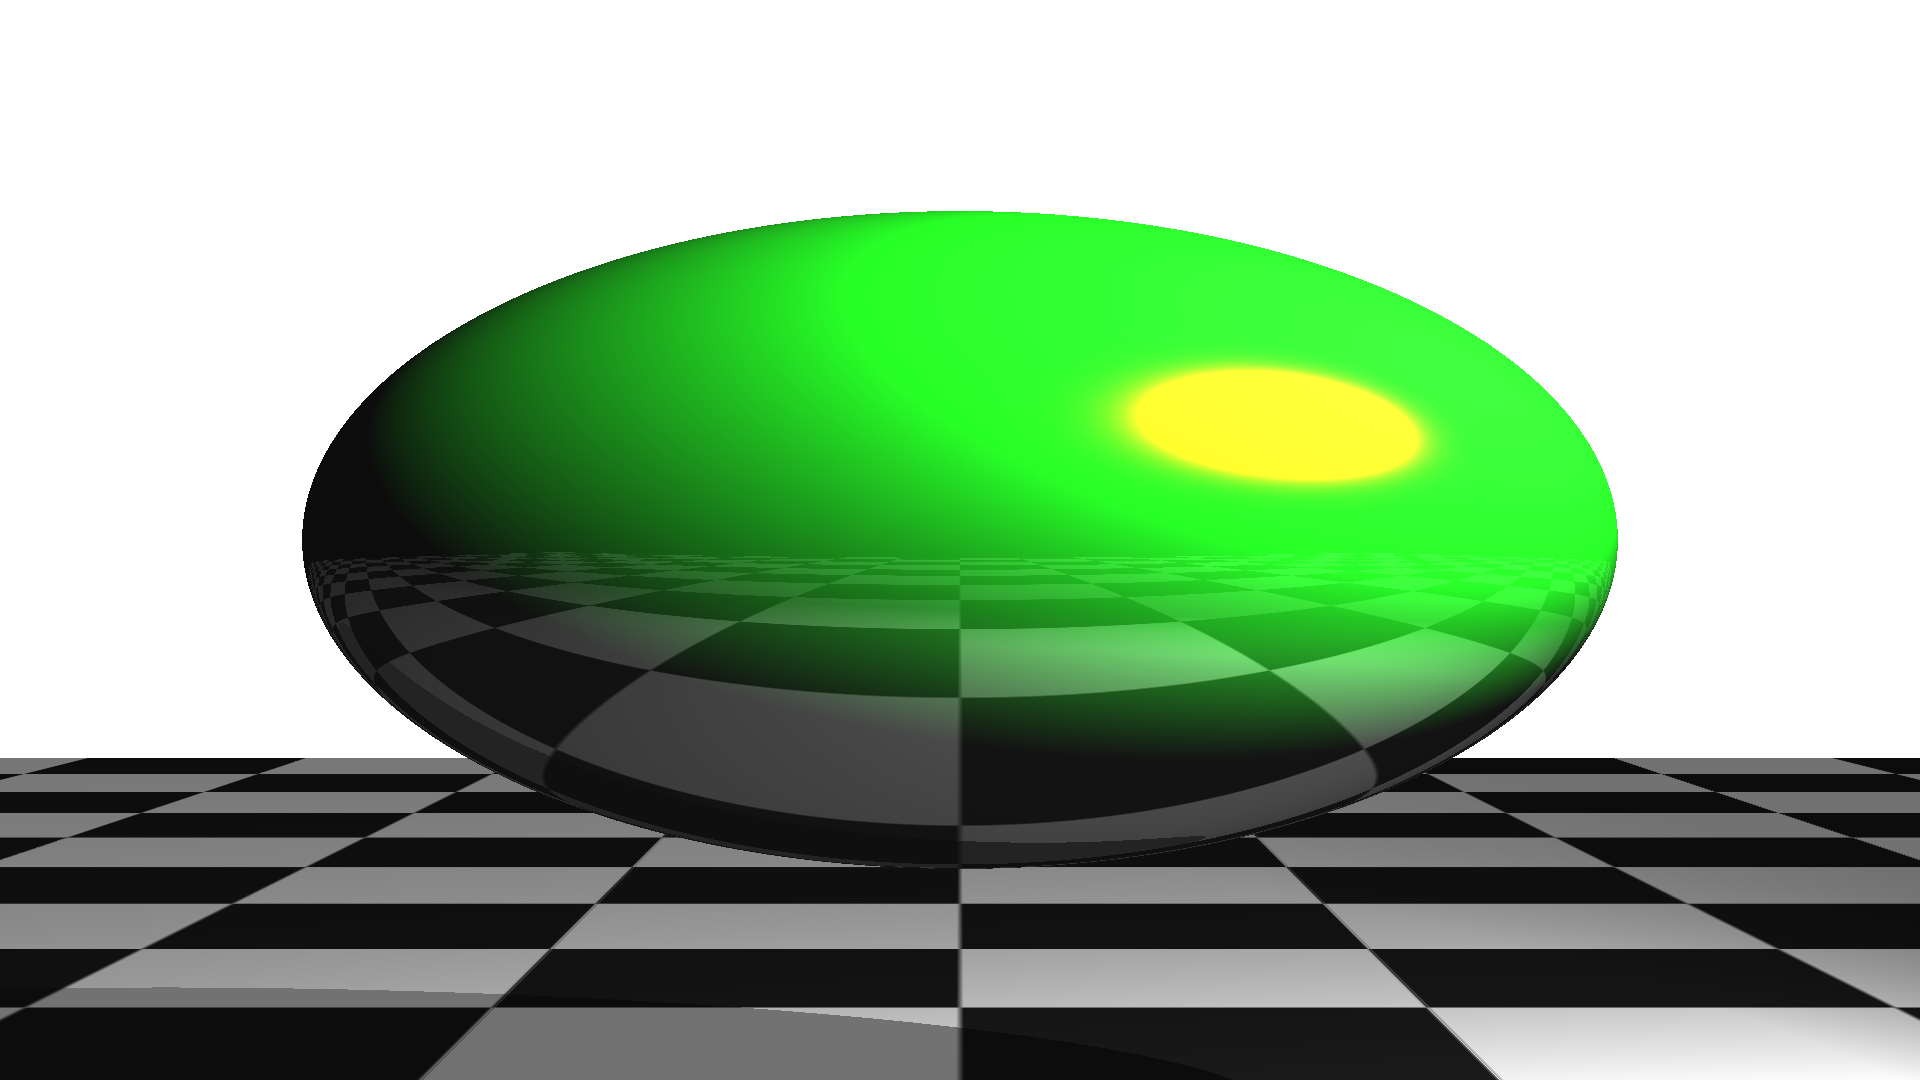
\includegraphics[width=0.3\textwidth]{chapters/ch3/img/reflection/specular_ks_02.png}}
\subfigure{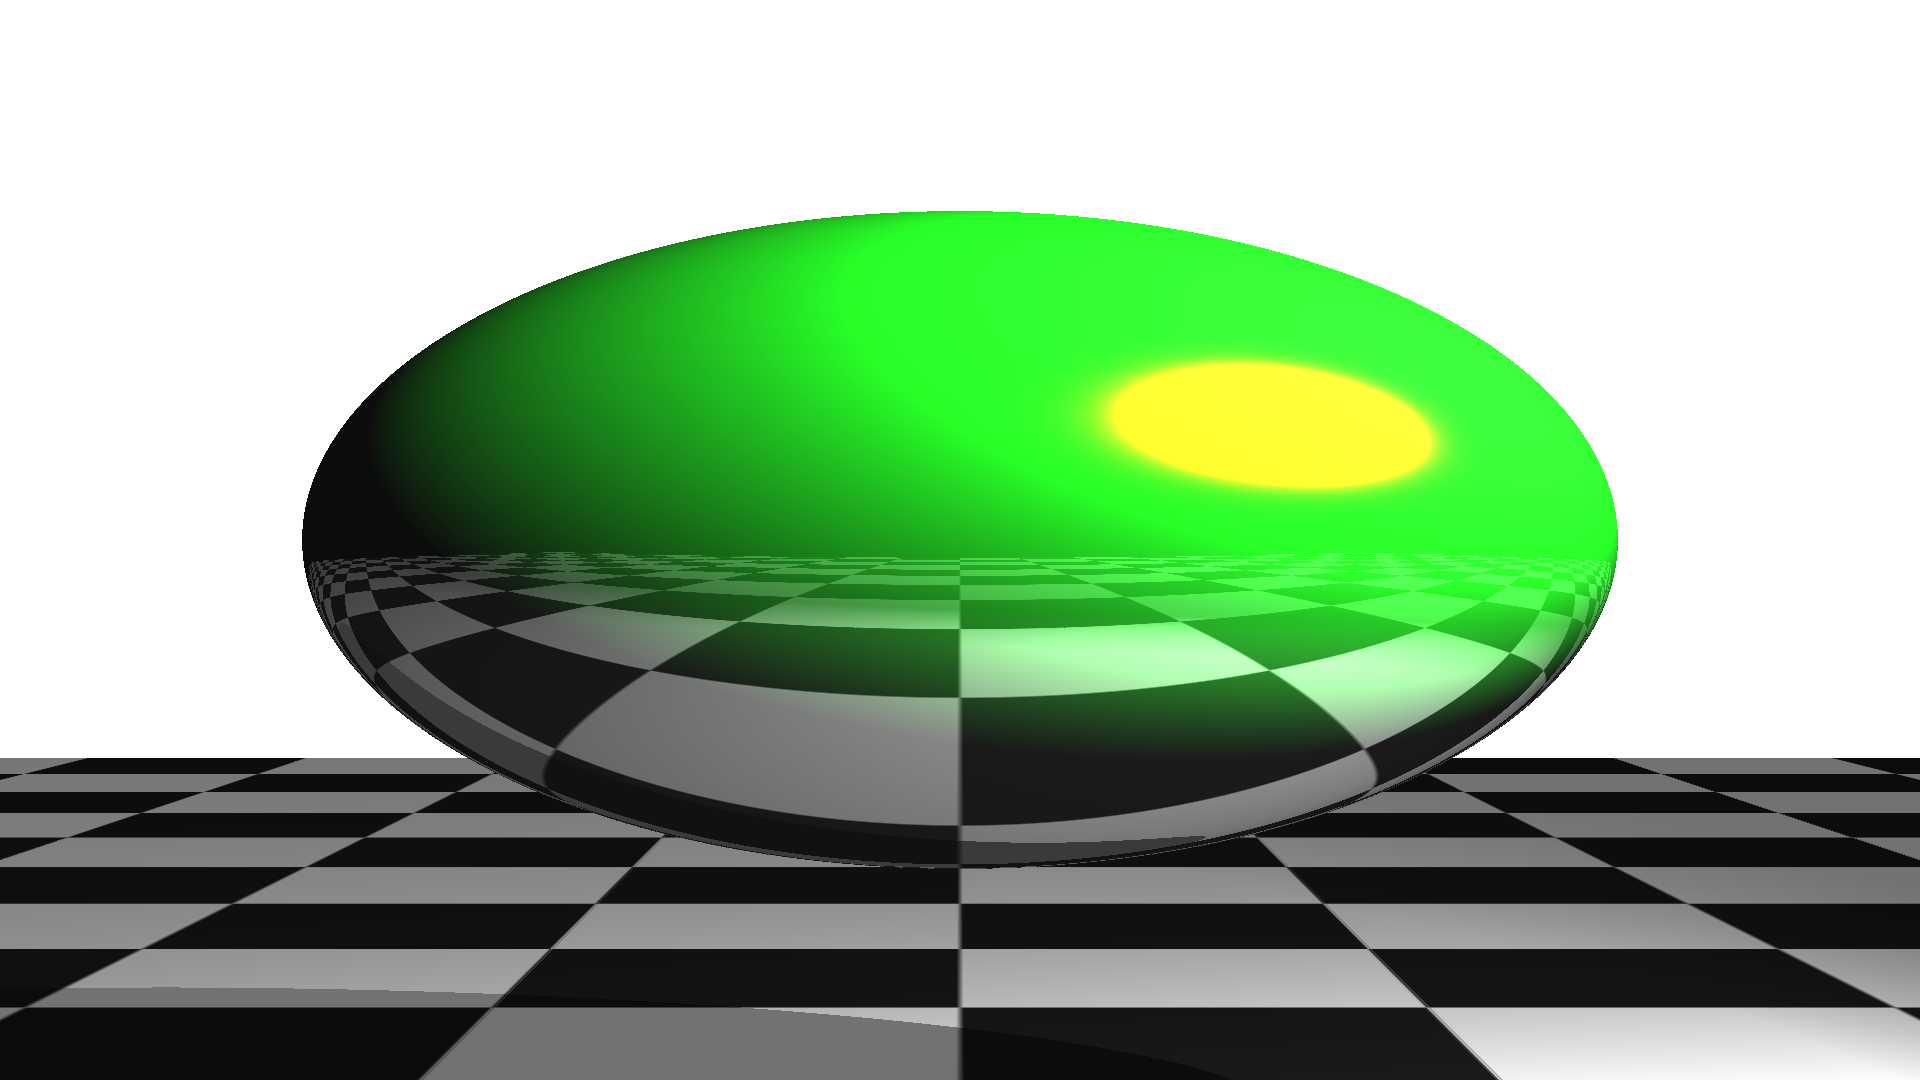
\includegraphics[width=0.3\textwidth]{chapters/ch3/img/reflection/specular_ks_04.png}}
\subfigure{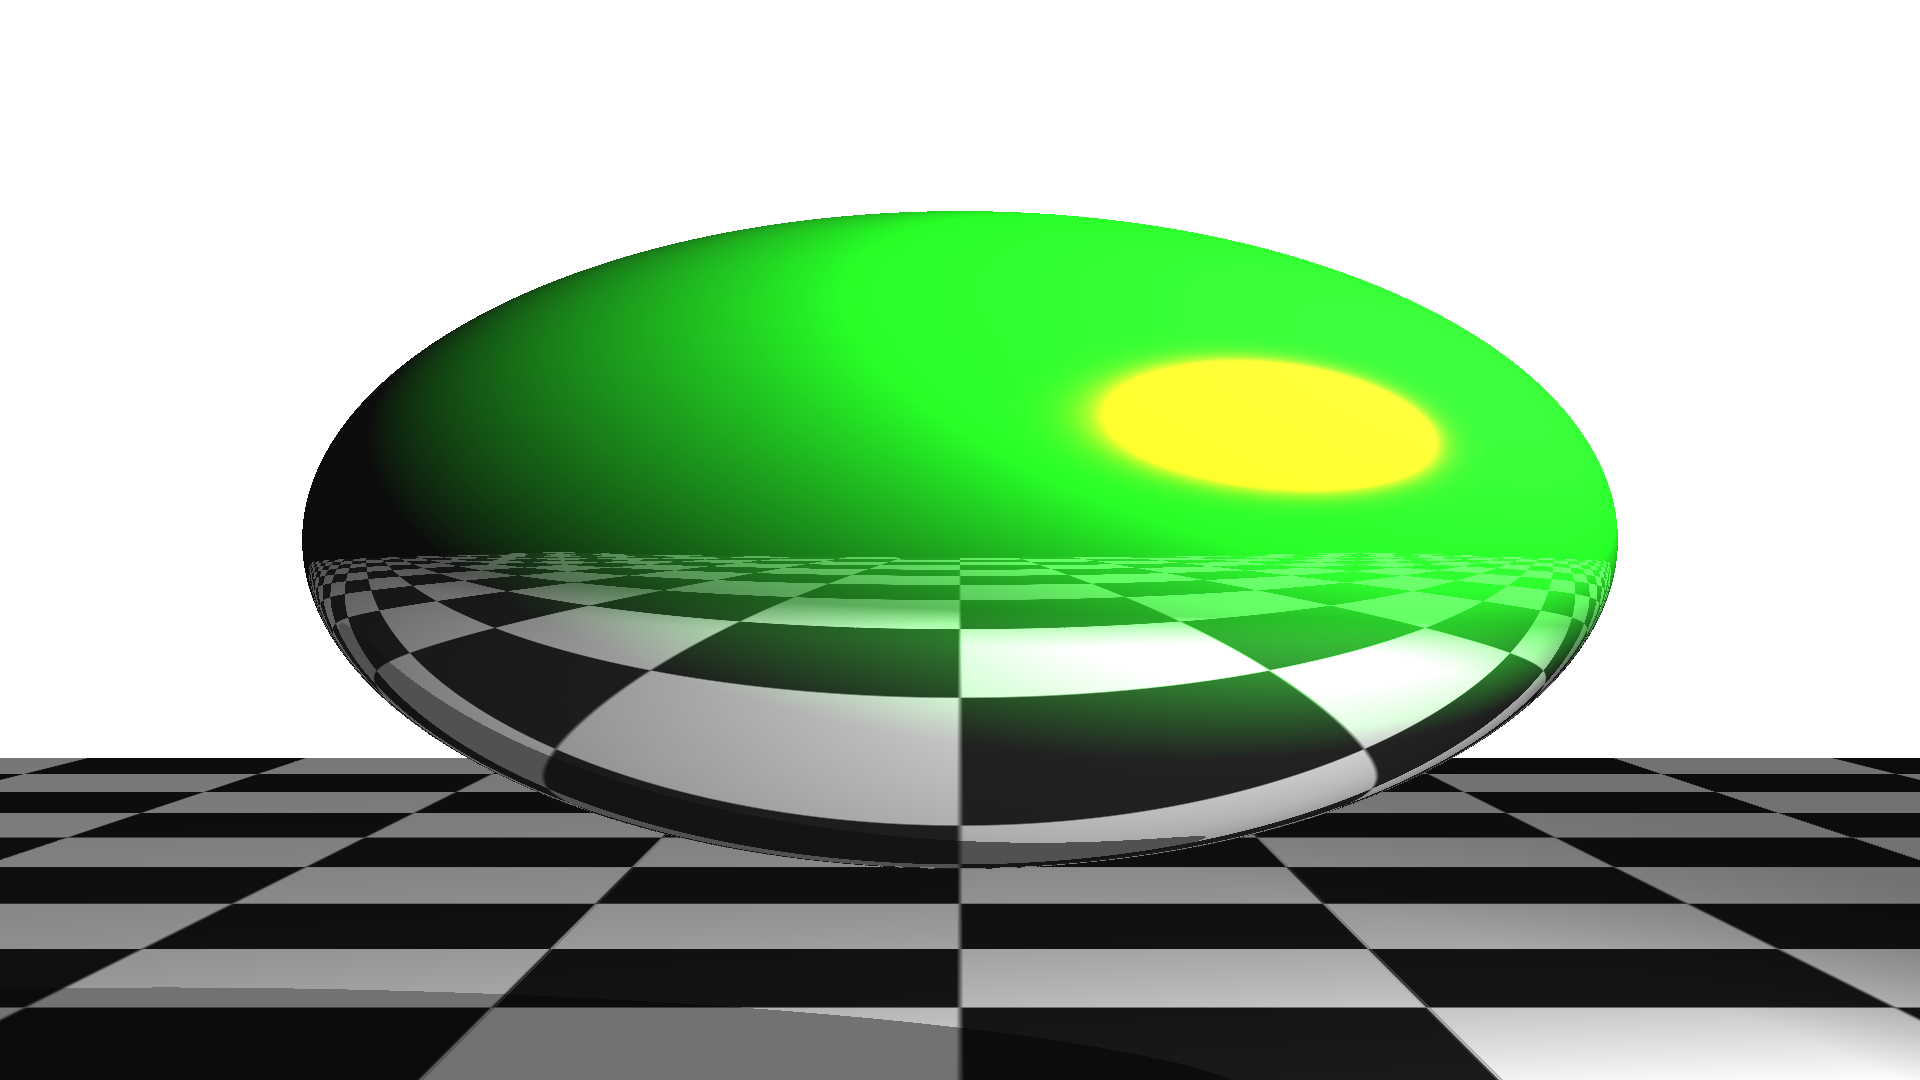
\includegraphics[width=0.3\textwidth]{chapters/ch3/img/reflection/specular_ks_06.png}}
\caption[Powierzchnie odbijające w sposób lustrzany]{Powierzchnie odbijające w sposób lustrzany w modelu Blinna-Phonga. Współczynnik odbicia $r_{l-1}$ jest stały, niezależny od kąta padania na płaszczyznę elipsoidy i równy współczynnikowi $k_s\in\lbrace 0,2; 0,4; 0,6 \rbrace$~($k_s$ rośnie od lewej do prawej)}
\label{ch3:img:reflection_types_specular}
\end{figure}

\begin{figure}[H]
\centering
\subfigure{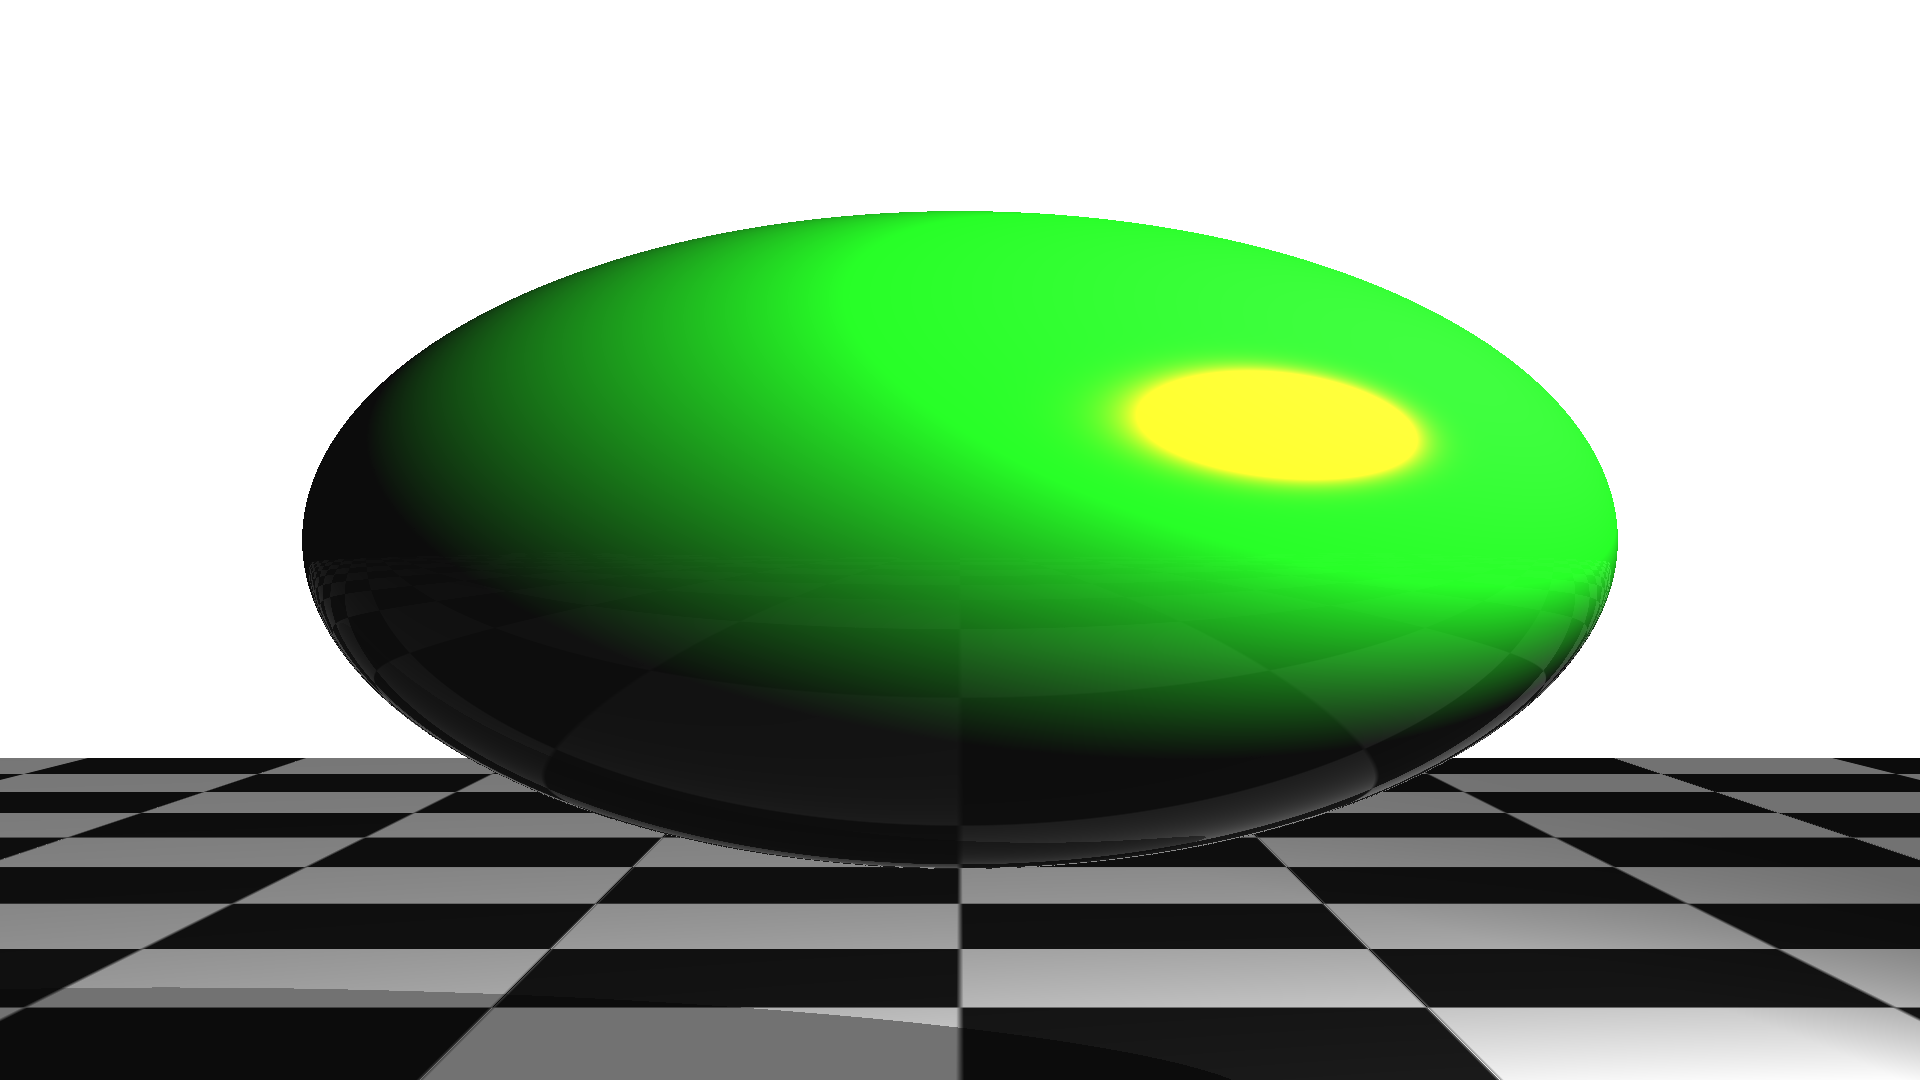
\includegraphics[width=0.3\textwidth]{chapters/ch3/img/reflection/fresnel_ks_02_exp_128_eta_133.png}}
\subfigure{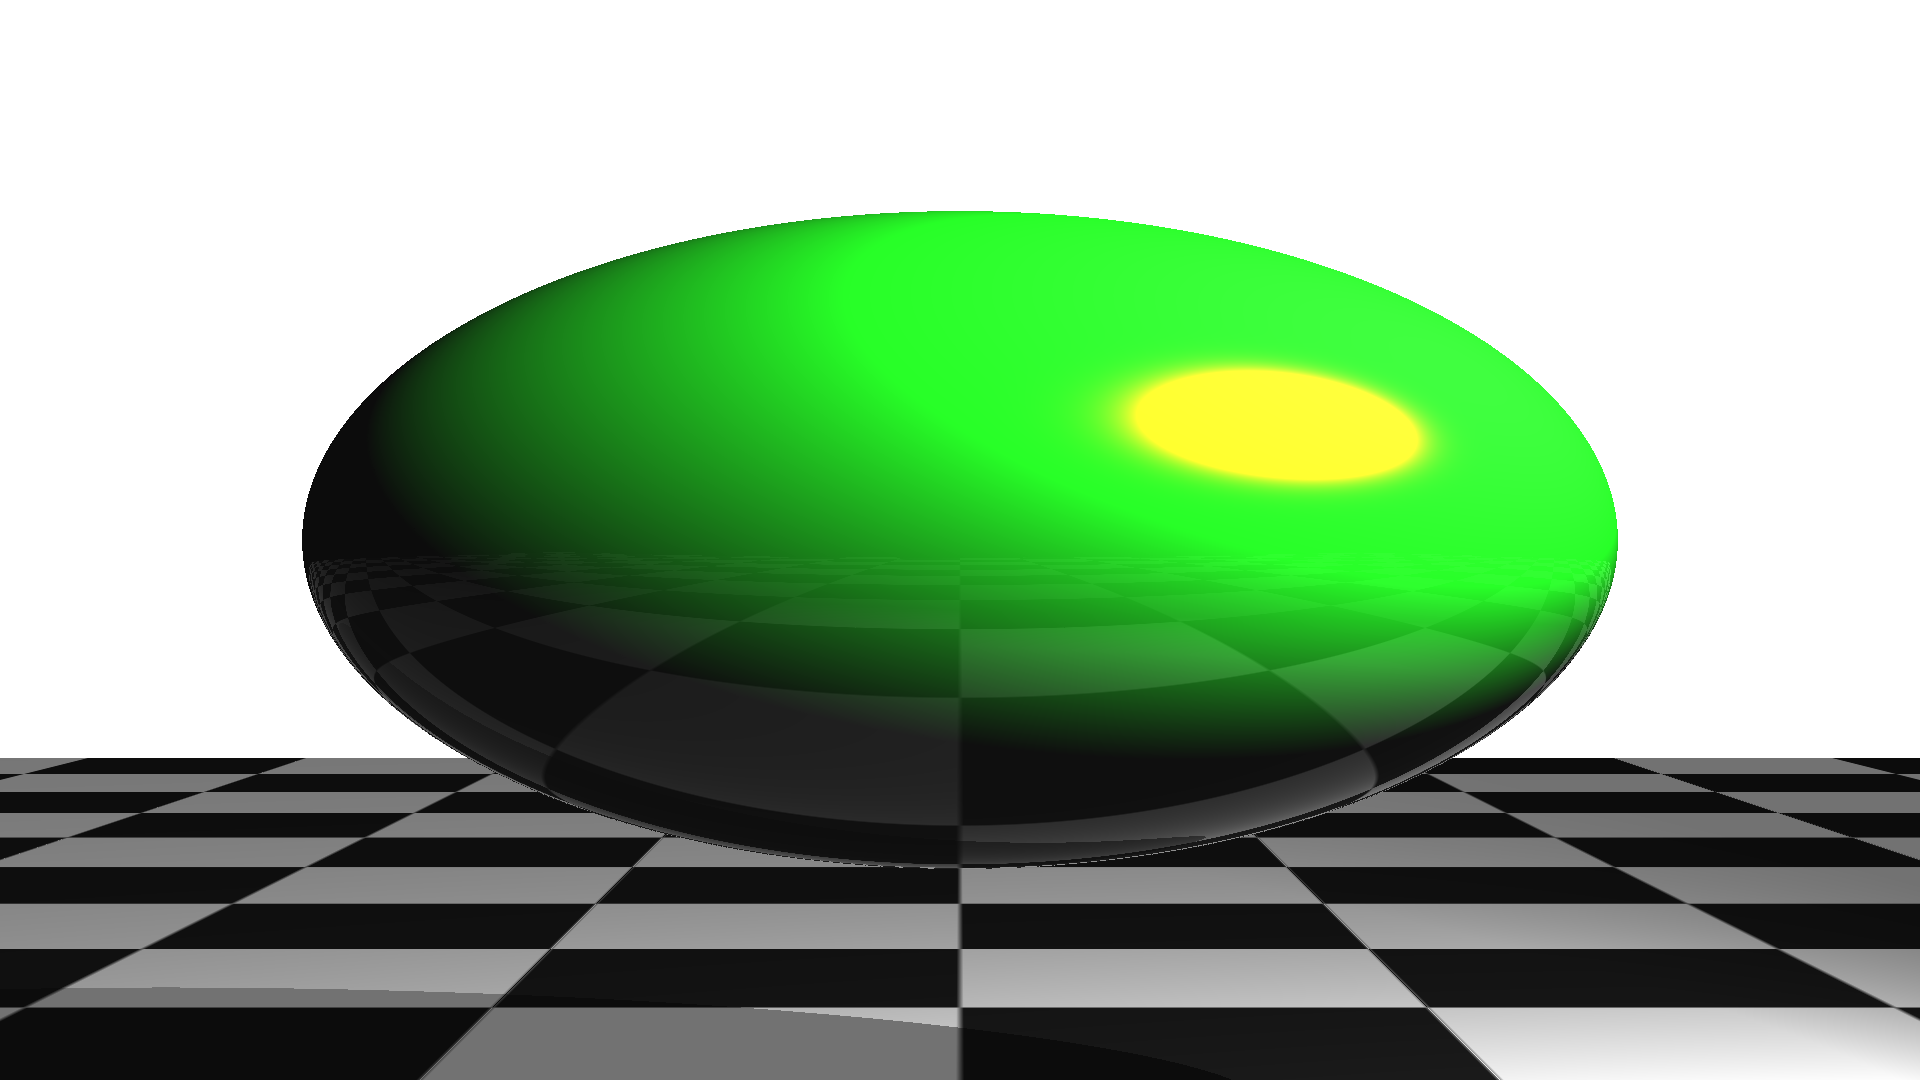
\includegraphics[width=0.3\textwidth]{chapters/ch3/img/reflection/fresnel_ks_02_exp_128_eta_166.png}}
\subfigure{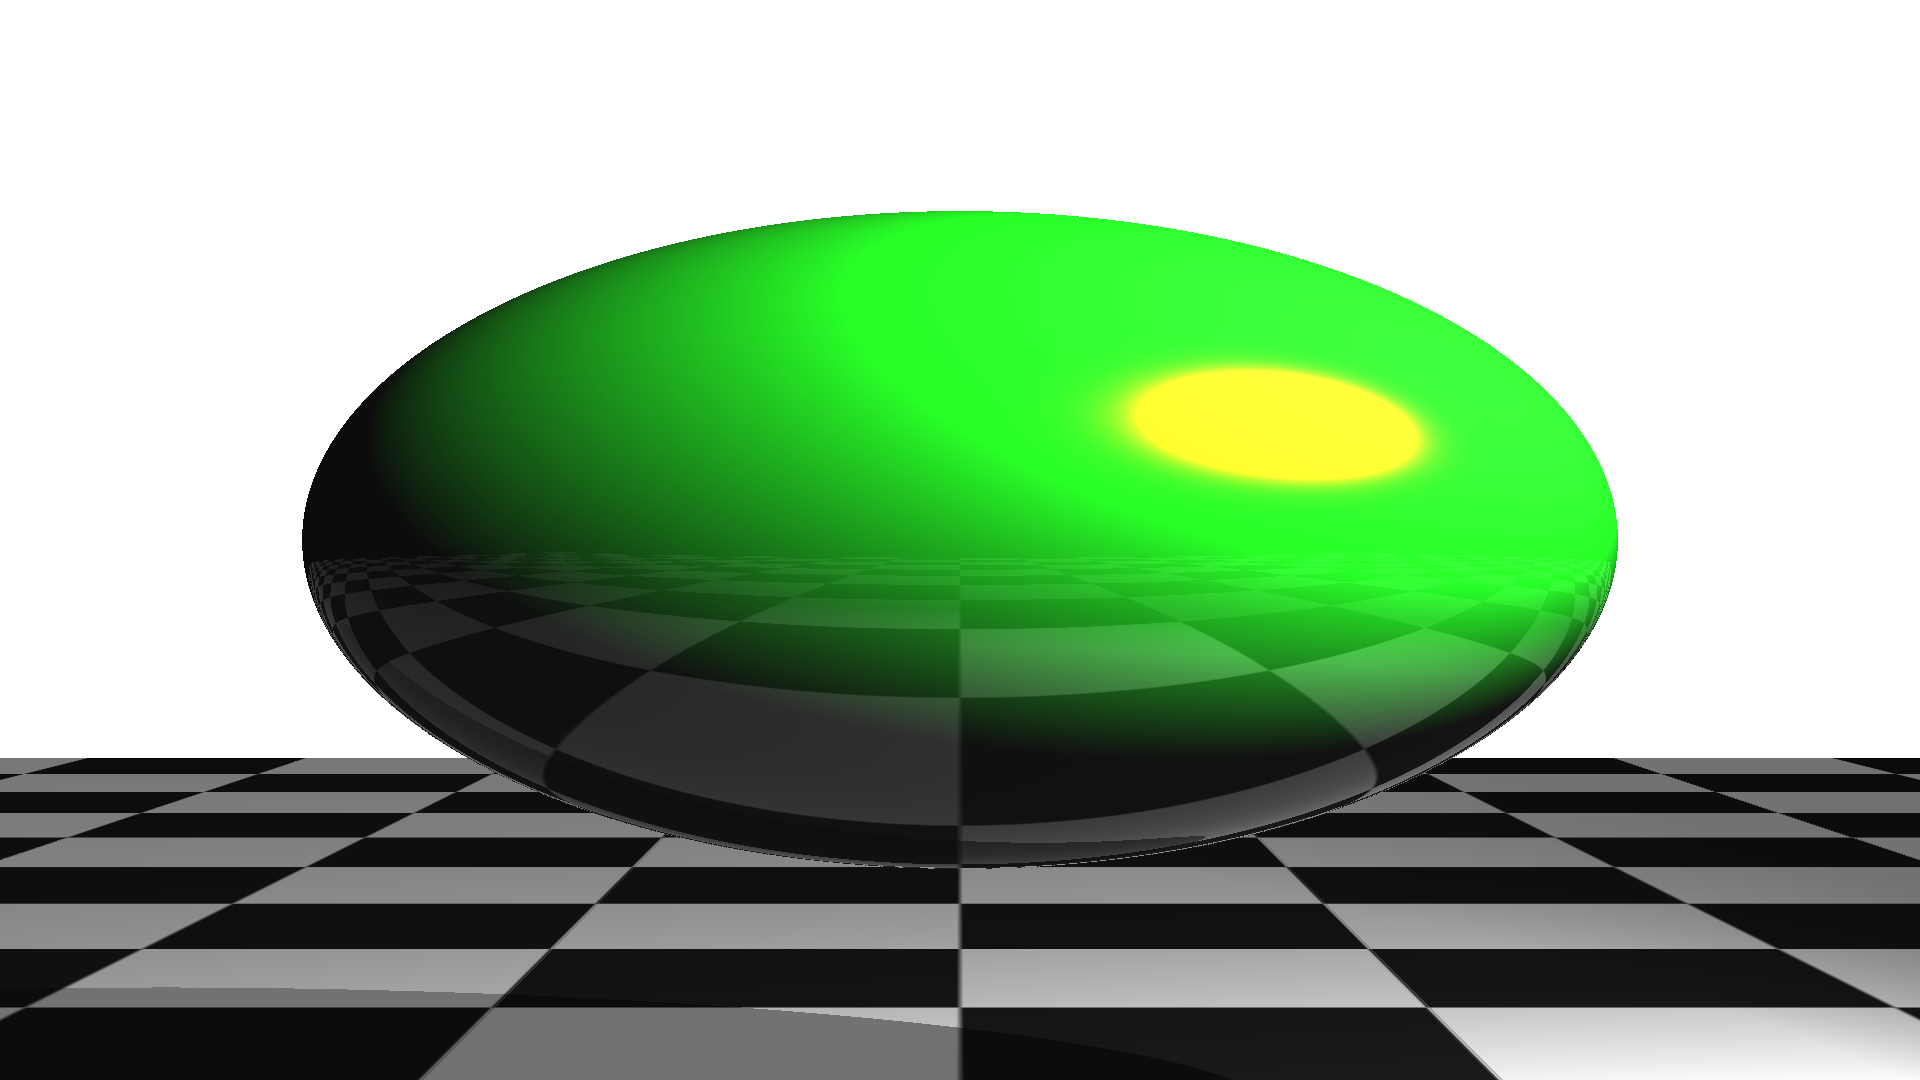
\includegraphics[width=0.3\textwidth]{chapters/ch3/img/reflection/fresnel_ks_02_exp_128_eta_200.png}}

\subfigure{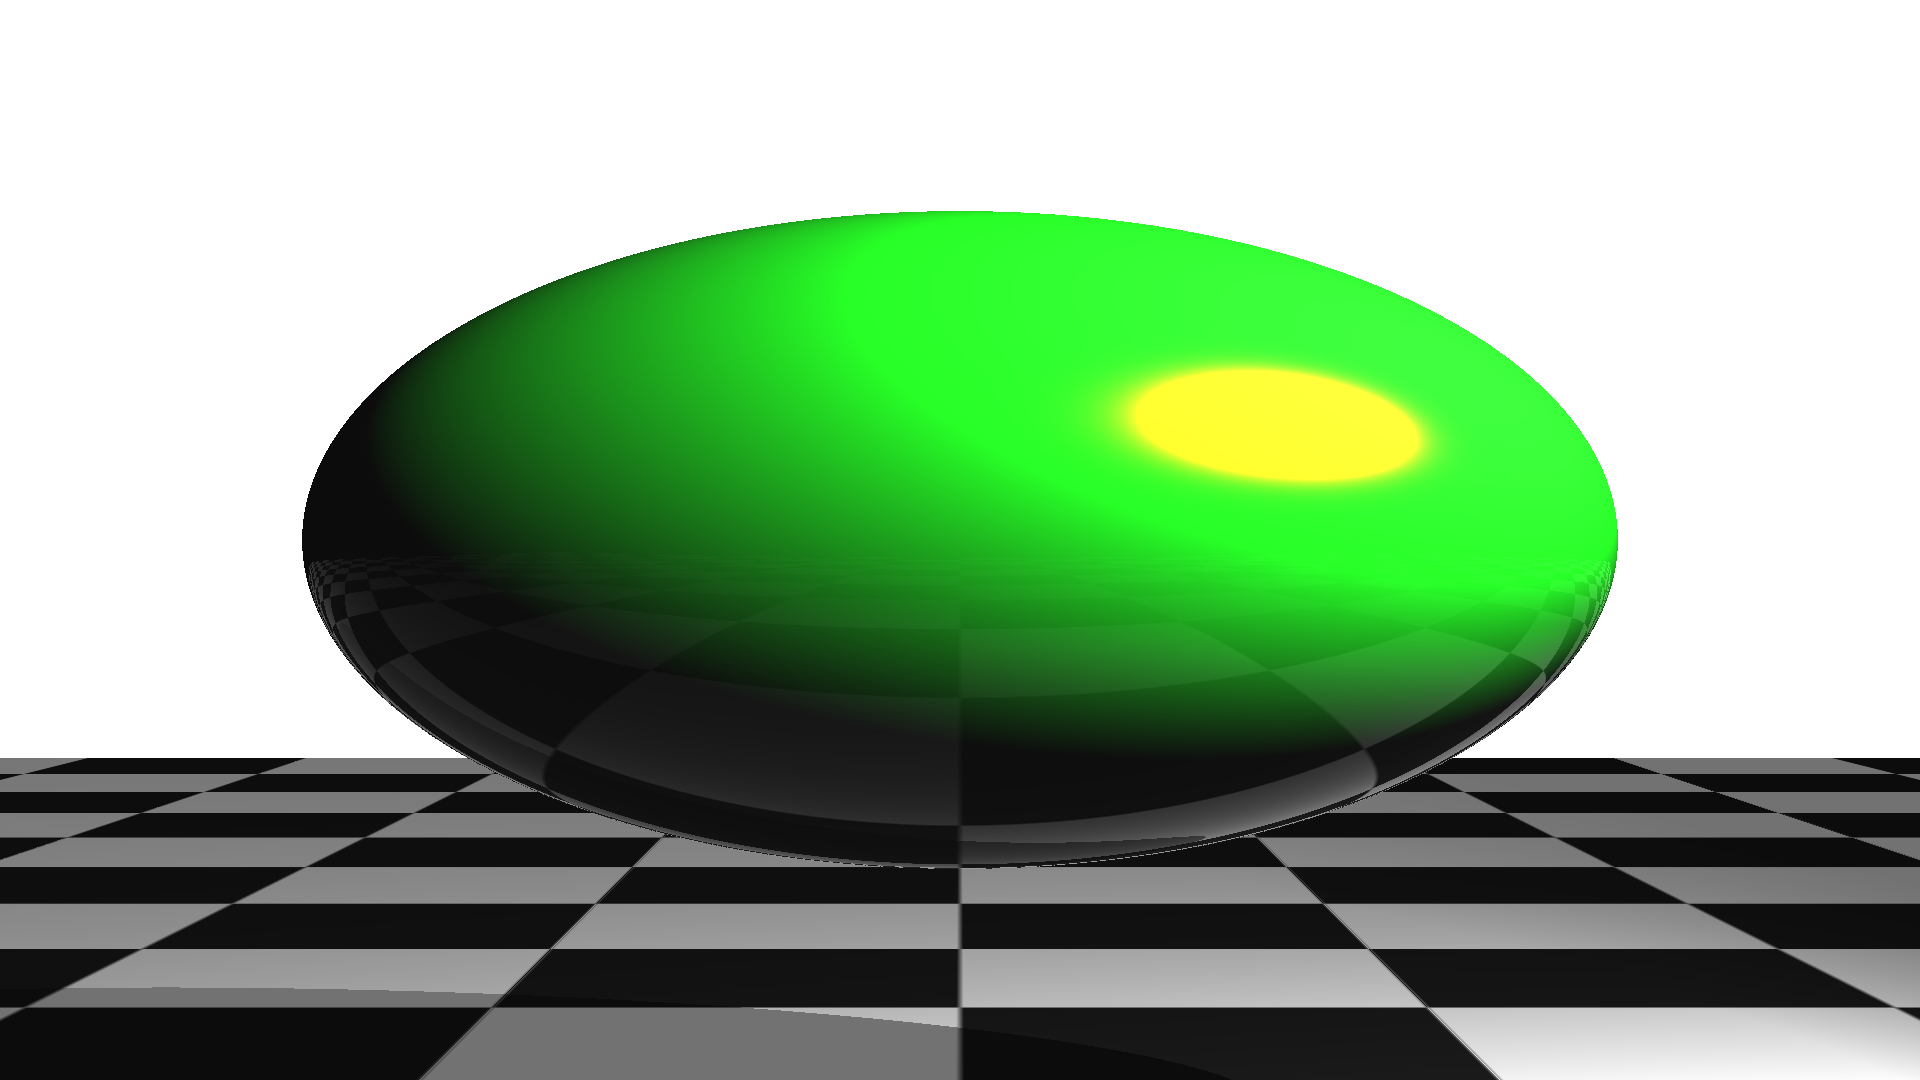
\includegraphics[width=0.3\textwidth]{chapters/ch3/img/reflection/fresnel_ks_02_exp_128_eta_133_k_02.png}}
\subfigure{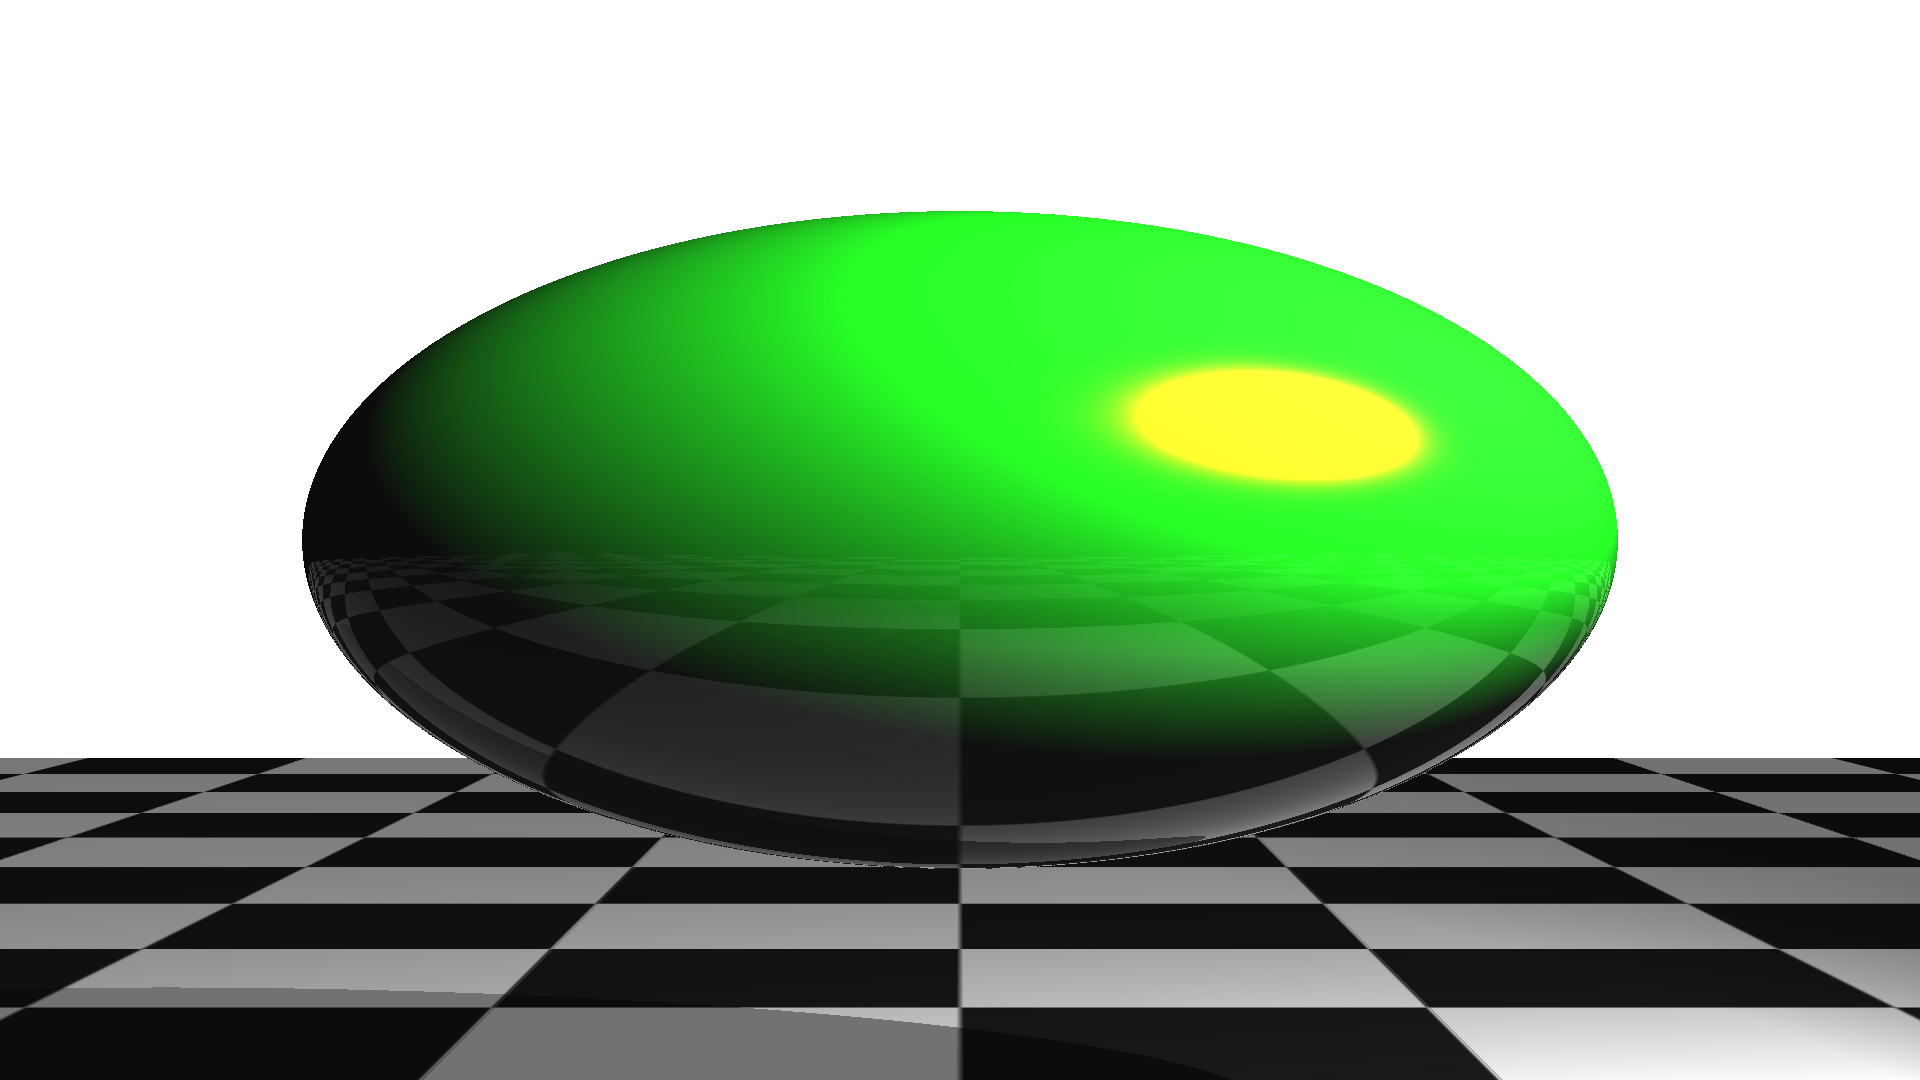
\includegraphics[width=0.3\textwidth]{chapters/ch3/img/reflection/fresnel_ks_02_exp_128_eta_133_k_06.png}}
\subfigure{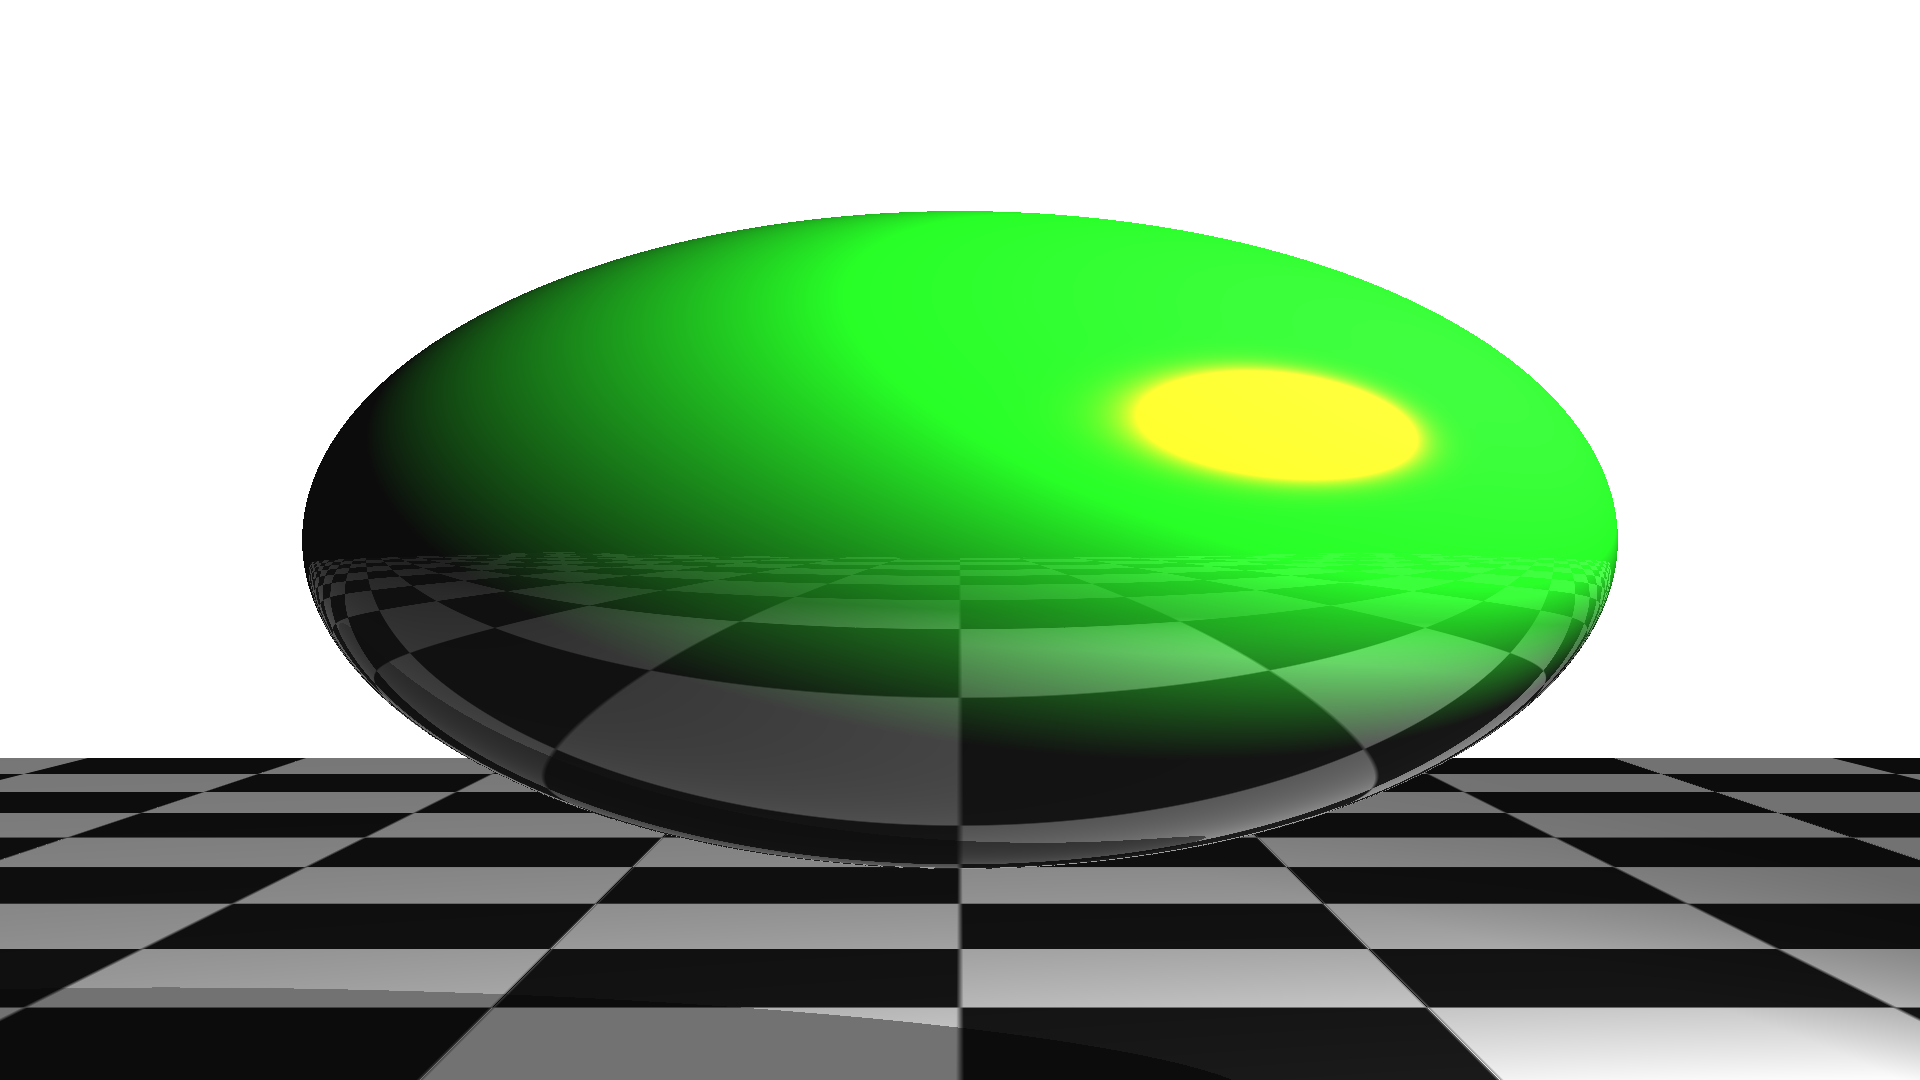
\includegraphics[width=0.3\textwidth]{chapters/ch3/img/reflection/fresnel_ks_02_exp_128_eta_133_k_10.png}}
\caption[Powierzchnie odbijające zgodnie ze wzorami Fresnela]{Powierzchnie odbijające zgodnie ze wzorami Fresnela w modelu Blinna-Phonga. Obrazy w górnym wierszu odpowiadają dielektrykom~($k=0$) o współczynniku załamania (od lewej do prawej) $\eta\in\lbrace 1,33; 1,66; 2,00 \rbrace$. Dla najmniejszego ze współczynników załamania $\eta=1,33$ odbicia są słabo zauważalne, jednak $r_{l-1}$ rośnie bardzo szybko, gdy promień padający staje się styczny do powierzchni. W dolnym wierszu przedstawione zostały przewodniki o~$k\in\lbrace 0,2; 0,6; 1,0 \rbrace$ i $\eta = 1,33$, których powierzchnie są znacznie bardziej odbijające niż w~przypadku dielektryka o tym samym $\eta$}
\label{ch3:img:reflection_types_fresnel}
\end{figure}

Zastosowanie modelu Torrance'a-Sparrowa na rysunku~\ref{ch3:img:reflection_types_ts} zamiast modelu Blinna-Phonga z odbiciem Fresnela~(rysunek~\ref{ch3:img:reflection_types_fresnel}) wprowadza dwie główne zmiany w obrazie:
\begin{enumerate}
\item Siła rozbłysku w prawej górnej części elipsoidy jest mniejsza i należy stosować większy współczynnik skupienia $e$.
\item Współczynnik odbicia, ze względu na sposób jego określenia w modelu Torrance'a-Sparrowa między wektorem połówkowym $\vec{\omega_h}$ a $\vec{\omega_o}$, nie rośnie tak szybko wraz ze~wzrostem kąta padania.   
\end{enumerate}

\begin{figure}[H]
\centering

\subfigure{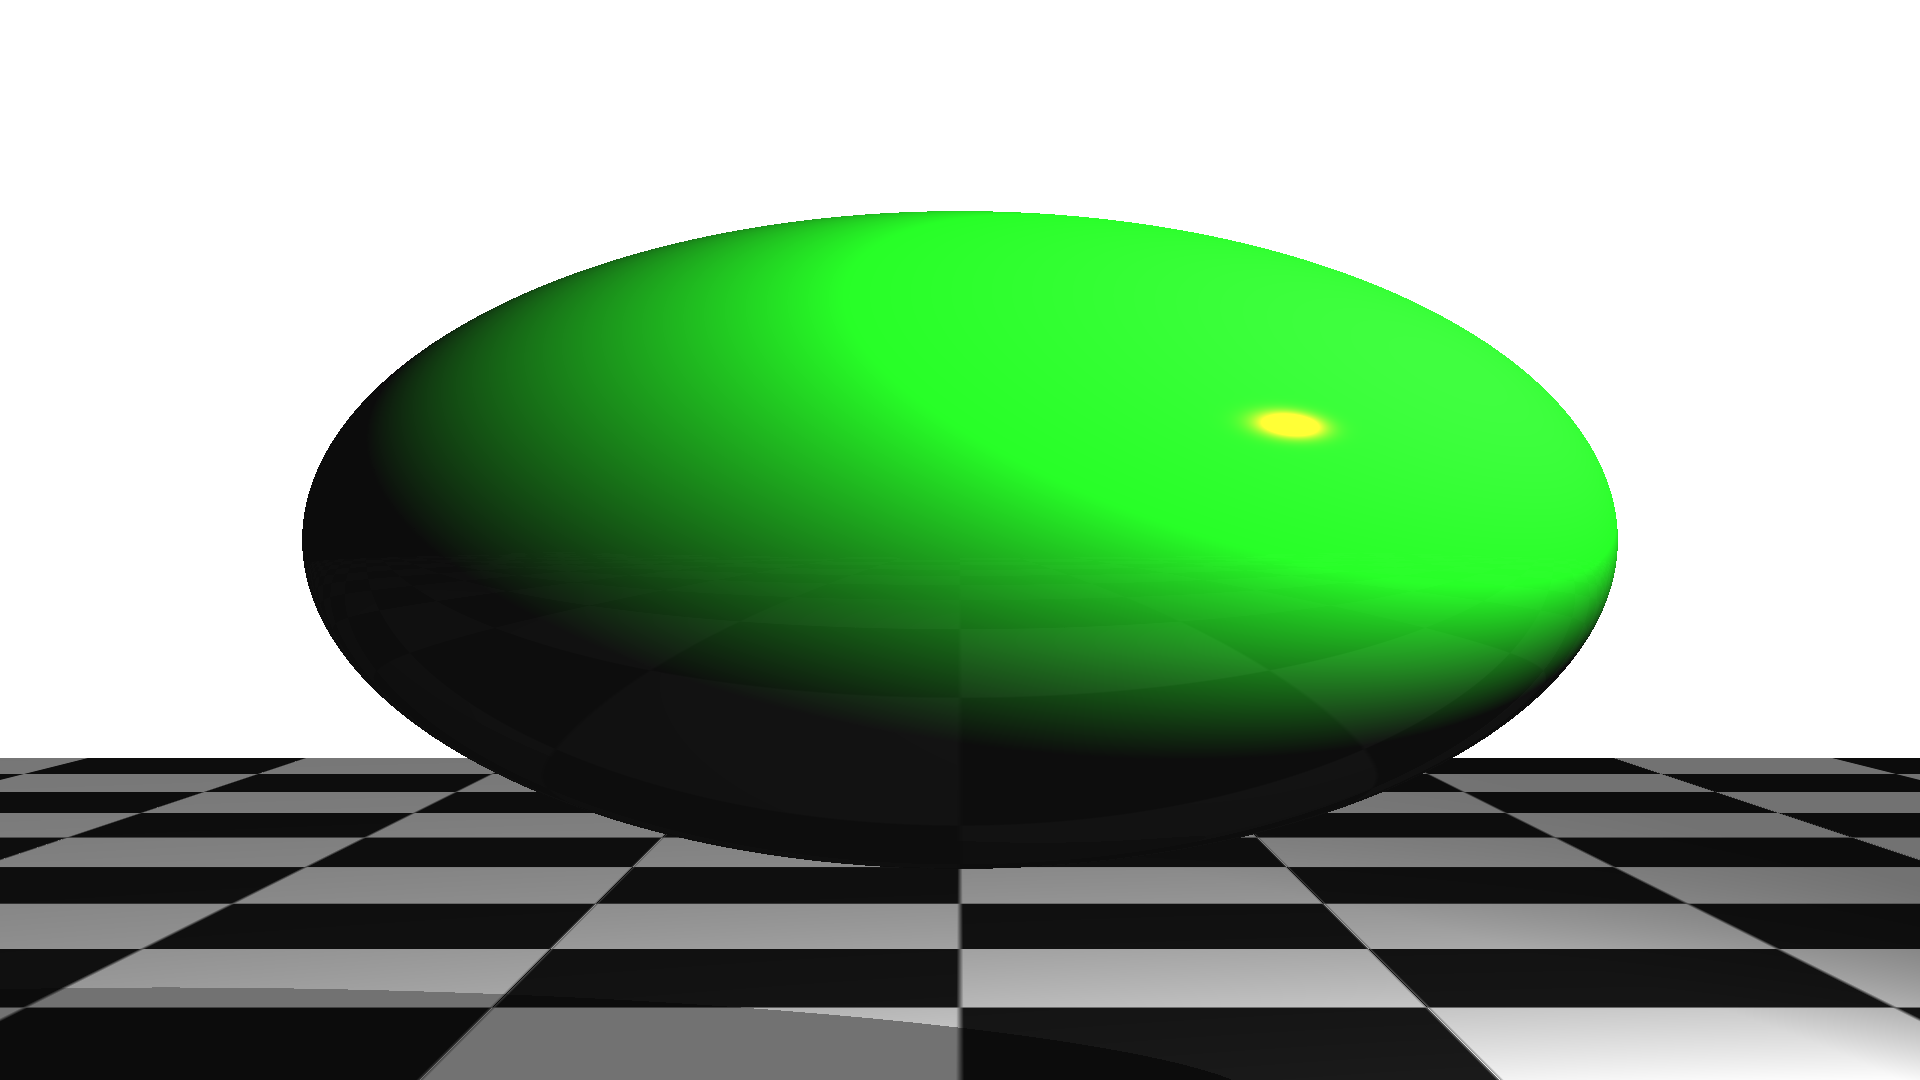
\includegraphics[width=0.3\textwidth]{chapters/ch3/img/reflection/ts_ks_06_exp_1024_eta_133.png}}
\subfigure{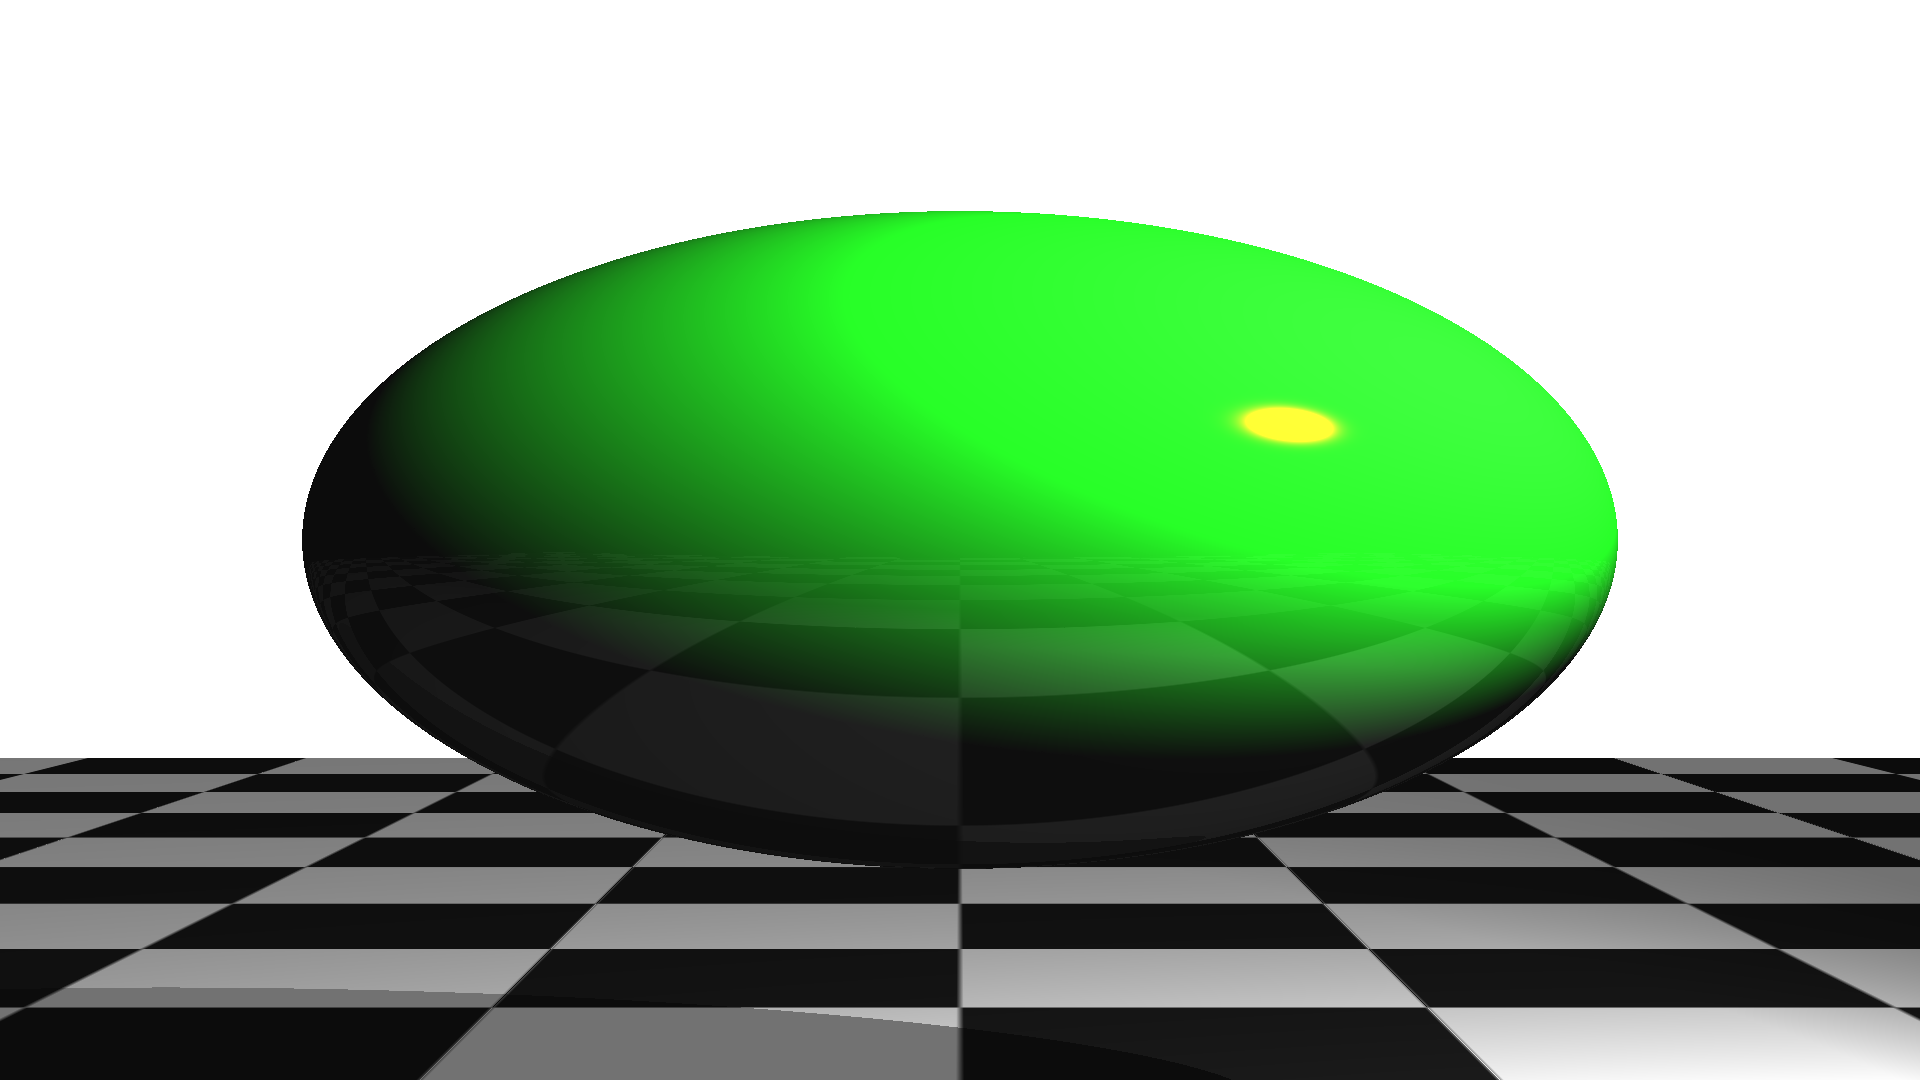
\includegraphics[width=0.3\textwidth]{chapters/ch3/img/reflection/ts_ks_06_exp_1024_eta_166.png}}
\subfigure{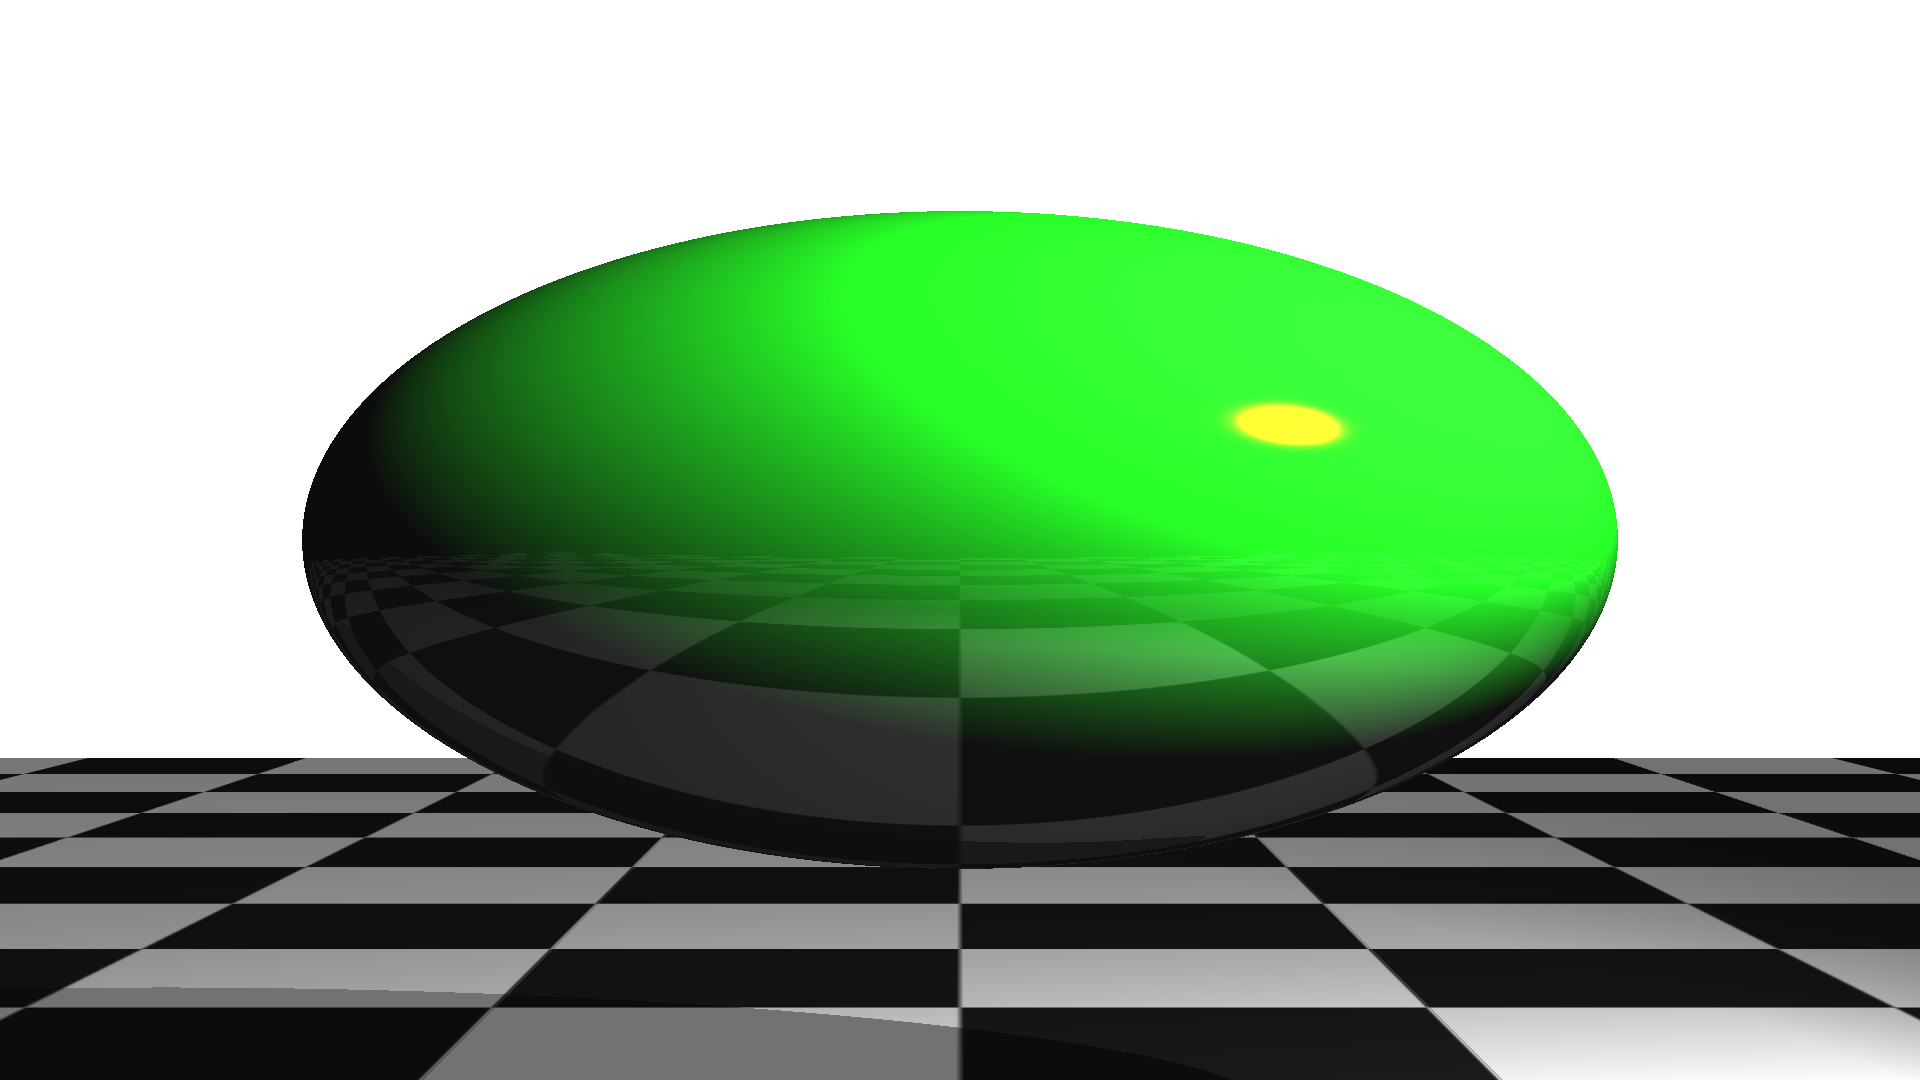
\includegraphics[width=0.3\textwidth]{chapters/ch3/img/reflection/ts_ks_06_exp_1024_eta_200.png}}

\subfigure{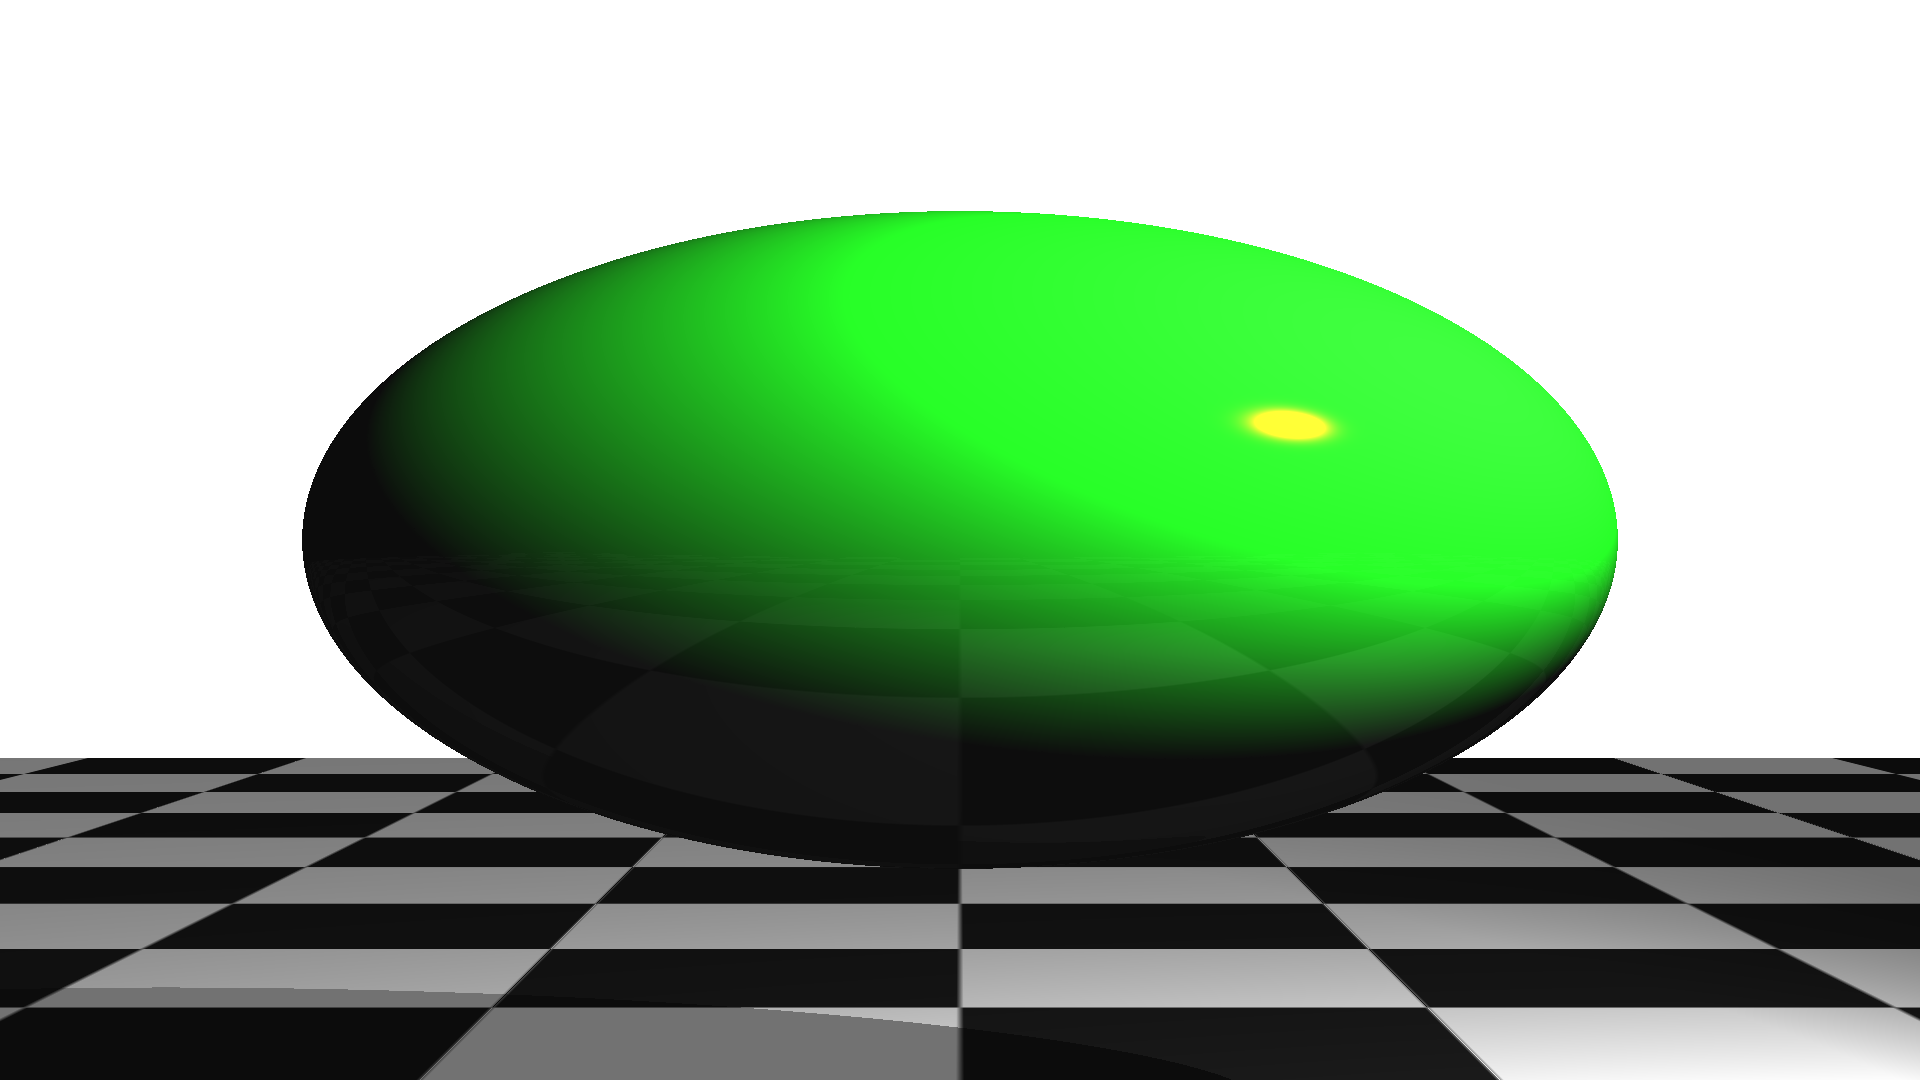
\includegraphics[width=0.3\textwidth]{chapters/ch3/img/reflection/ts_ks_06_exp_1024_eta_133_k_02.png}}
\subfigure{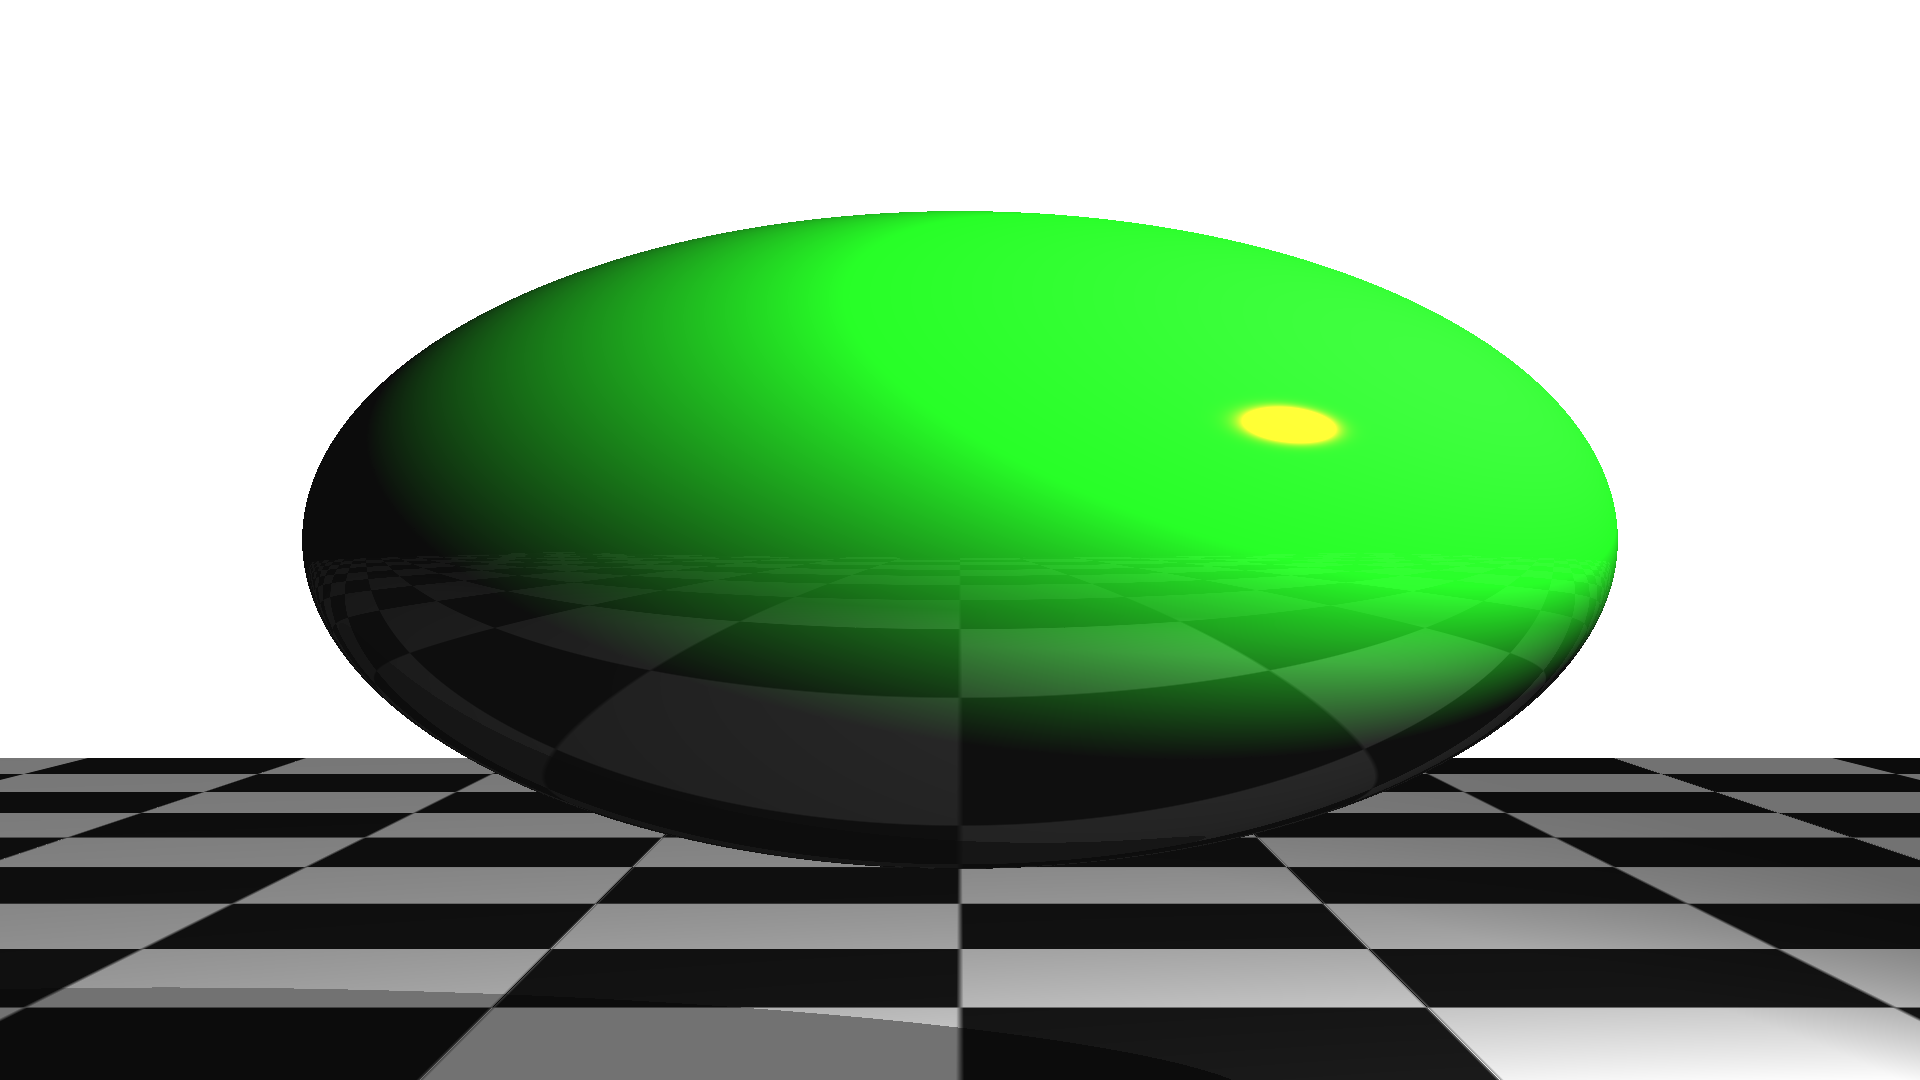
\includegraphics[width=0.3\textwidth]{chapters/ch3/img/reflection/ts_ks_06_exp_1024_eta_133_k_06.png}}
\subfigure{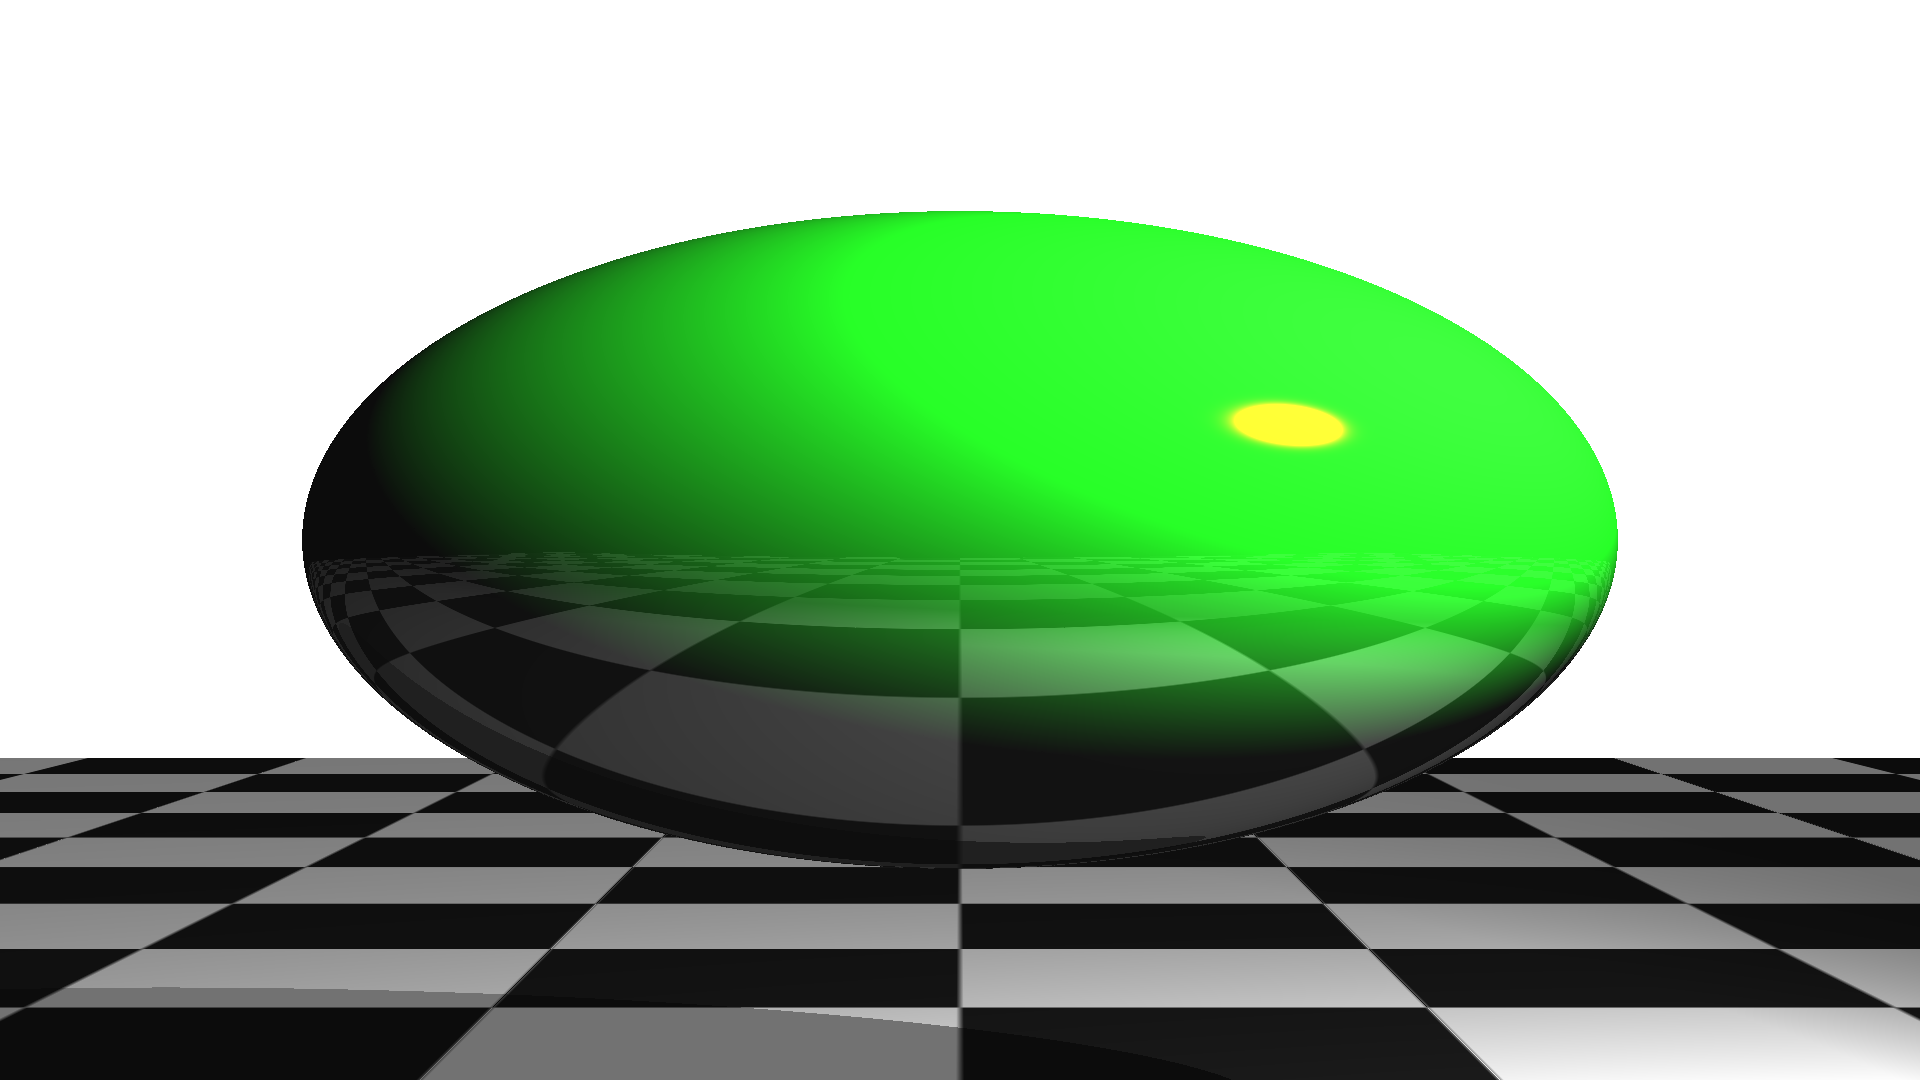
\includegraphics[width=0.3\textwidth]{chapters/ch3/img/reflection/ts_ks_06_exp_1024_eta_133_k_10.png}}

\caption[Powierzchnie odbijające w modelu Torrance'a-Sparrowa]{Powierzchnie odbijające w modelu Torrance'a-Sparrowa. Obrazy w górnym wierszu odpowiadają dielektrykom~($k=0$) o współczynniku załamania (od lewej do prawej) $\eta\in\lbrace 1,33; 1,66; 2,00 \rbrace$. W dolnym wierszu przedstawione zostały przewodniki o~$k\in\lbrace 0,2; 0,6; 1,0 \rbrace$ i $\eta = 1,33$}
\label{ch3:img:reflection_types_ts}
\end{figure}
